\documentclass[11pt,a4paper]{article}

% ---------------------------------------------------------------------------
% Gigalis internship report -- Executive / orientation document.
% For implementation details, diagnostics, and methodology see
% phase1_technical_report.tex / phase1_technical_report.pdf.
% For data-reliability and event-definition detail see data_quality_report.
% ---------------------------------------------------------------------------

\usepackage[utf8]{inputenc}
\usepackage[T1]{fontenc}
\usepackage{amsmath}
\usepackage{booktabs}
\usepackage{geometry}
\usepackage{graphicx}
\usepackage{pdflscape}
\usepackage{caption}
\usepackage{subcaption}
\usepackage{float}
\usepackage{xcolor}
\usepackage{enumitem}
\usepackage{fancyhdr}
\usepackage{xurl}
\usepackage[hidelinks]{hyperref}

\geometry{margin=2.3cm}
\setlength{\parskip}{0.5em}
\setlength{\parindent}{0pt}
\setlength{\emergencystretch}{3em}
\captionsetup{font=small,labelfont=bf}

\definecolor{darkblue}{RGB}{0,51,102}
\definecolor{done}{RGB}{0,120,50}
\definecolor{partial}{RGB}{180,100,0}
\definecolor{notdone}{RGB}{160,0,0}
\hypersetup{colorlinks=true,linkcolor=darkblue,urlcolor=darkblue,citecolor=darkblue}

\pagestyle{fancy}
\fancyhf{}
\rhead{\small Gigalis Internship --- Orientation Report}
\lhead{\small Predictive Procurement Modeling}
\cfoot{\thepage}
\setlength{\headheight}{14pt}

\title{\textbf{Predicting Contract Renewal in Public Digital Procurement}\\[0.4em]
      \large A Survival-Analysis Approach on BOAMP Notices for Gigalis\\[0.3em]
      \normalsize Internship Report --- Executive Orientation}
\author{Internship Report --- Gigalis (Pays de la Loire)}
\date{June 2026}

\begin{document}
\maketitle
\thispagestyle{fancy}

% ===========================================================================
\begin{abstract}
\noindent
This is the \textbf{executive report} of the internship: it lets a reader scan
the project rapidly and understand \emph{what was done}, \emph{why it matters},
and \emph{what is reliable}. The full implementation and diagnostics are in the
\textbf{technical report} (\texttt{phase1\_technical\_report.pdf}); the data
reliability and event-definition detail are in the \textbf{data quality report}.

The work concerns predictive analysis of public digital procurement for
\textbf{Gigalis}, a central purchasing body in Pays de la Loire. The goal is to
move from a descriptive view (``what happened?'') towards a predictive one
(``when will a contract be re-tendered?''). Because BOAMP contains \emph{no
explicit renewal field}, the renewal relationship is reconstructed from
observable signals: a proxy renewal \texttt{event} built from
Sentence-Transformer text embeddings combined with CPV, temporal, and buyer
signals, used as the event variable for survival analysis. On 1{,}210 eligible
source contracts the linking method recovers a plausible renewal for 665 of them
(\textbf{55.0\%}), against a 7.6\% lexical baseline at the same window setting. Survival modeling gives a
global Kaplan--Meier median survival of \textbf{50.1 months}, a Cox concordance
of \textbf{0.6317}, and a best-fitting log-normal parametric model (AIC
7{,}068.4). The fitted model is translated into 12- and 24-month renewal-risk
indicators at contract, buyer, and segment level. Buyer identities were
consolidated by a SIREN enrichment step (completed 2026-06-24). The headline
caveat: \texttt{event} is a proxy, and a manual audit of a stratified 150-case
sample (2026-07-02) estimates its precision at only $\approx$9--15\% overall ---
concentrated in the high-text-similarity core (precision 1.00 at text $\geq$0.80,
$\approx$0.50 in the HIGH/strict tier, $\approx$0 below composite 0.50). The
survival results should be read as describing algorithm-identifiable same-buyer
re-publications, not validated renewals. \textbf{This finding triggered a
methodological change}, described immediately below: the event definition was
recalibrated against a synthetic benchmark, trading linkage quantity for
analytical reliability (269 events, 22.2\%, rather than 665, 55.0\%).
\end{abstract}

\section*{Methodological Note --- From Maximizing Linkage to Maximizing Reliability (2026-07-05)}
\addcontentsline{toc}{section}{Methodological note --- calibration, 2026-07-05}

This note explains \emph{why} the event definition changed after the main
pipeline was first built, not just \emph{what} changed. It is the key to
reading the rest of this report: numbers in Section~\ref{sec:results} were
computed under the \textbf{initial} linking method; the numbers in this note
and in Section~\ref{sec:reliability} reflect the \textbf{calibrated} method
that should be used for any downstream decision.

\paragraph{Initial method and its results.}
The first version of the pipeline (Section~\ref{sec:linking}) linked a source
contract to \emph{any} later same-buyer notice whose composite score was
non-negative after passing a soft text-similarity filter. This maximized the
linking rate: 665 of 1{,}210 eligible contracts (55.0\%) were linked, against a
7.6\% lexical baseline --- a large apparent improvement.

\paragraph{Challenge discovered.}
BOAMP has no official field certifying that one notice renews another, so this
55.0\% figure could not be checked against ground truth directly. A manual
audit of 150 stratified cases against the full official BOAMP record
(2026-07-02) showed the initial rule was too permissive: raw precision was only
$\approx$0.15 (weighted $\approx$0.09 over the 665-event population), rising to
0.50 in the high-confidence tier and 1.00 only above text similarity 0.80; 12.8\%
of decided-unlinked sources also hid a plausible missed renewal. In short, the
initial rule optimized for \emph{linking rate}, not for \emph{link
correctness}, and there is no legal ground truth against which to prove any
individual link is right.

\paragraph{Reason for changing method.}
Because no certified renewal label exists for BOAMP, the true precision/recall
of any rule cannot be measured on the real data alone. The project therefore
stopped trying to maximize the number of linked events and instead built a
\textbf{synthetic BOAMP-like benchmark} with known recurrence truth by
construction, so that candidate rules could be compared on measurable
precision, recall, and F1 before being re-applied to real BOAMP. The goal
changed from \emph{``detect every true renewal''} to \emph{``construct a
reliable, calibrated proxy-event definition.''}

\paragraph{New calibrated method.}
The synthetic benchmark generates synthetic source notices, candidate notices,
and an explicit true-link table under three difficulty scenarios (easy,
medium, hard), with real-BOAMP-informed design parameters for timing,
buyer-name variation, generic or drifting CPV codes, missing duration/CPV,
short or paraphrased text, and large-buyer ambiguity. It is scored with the
\emph{same Sentence-Transformer encoder as the real pipeline}
(\nolinkurl{paraphrase-multilingual-MiniLM-L12-v2}), so benchmark performance is
directly comparable to the operational linking setup. A full threshold grid was
scored on the benchmark and three explicit rules were selected: \textbf{broad},
\textbf{balanced}, and \textbf{strict}. The recommended main rule is
\textbf{balanced}: text similarity $\geq 0.50$, composite score $\geq 0.50$,
temporal window $W=6$, corrected generic CPV scoring, no margin floor. On the
synthetic benchmark, the balanced rule scores precision/recall/F1 of
0.777/0.806/0.791 (easy), 0.601/0.586/0.593 (medium), and 0.318/0.302/0.310
(hard, Figure~\ref{fig:scenario-performance}) --- it was chosen over broad and
strict because it keeps acceptable reliability in the medium (realistic-noise)
scenario while still preserving enough real events for survival modeling.

\begin{figure}[H]
\centering
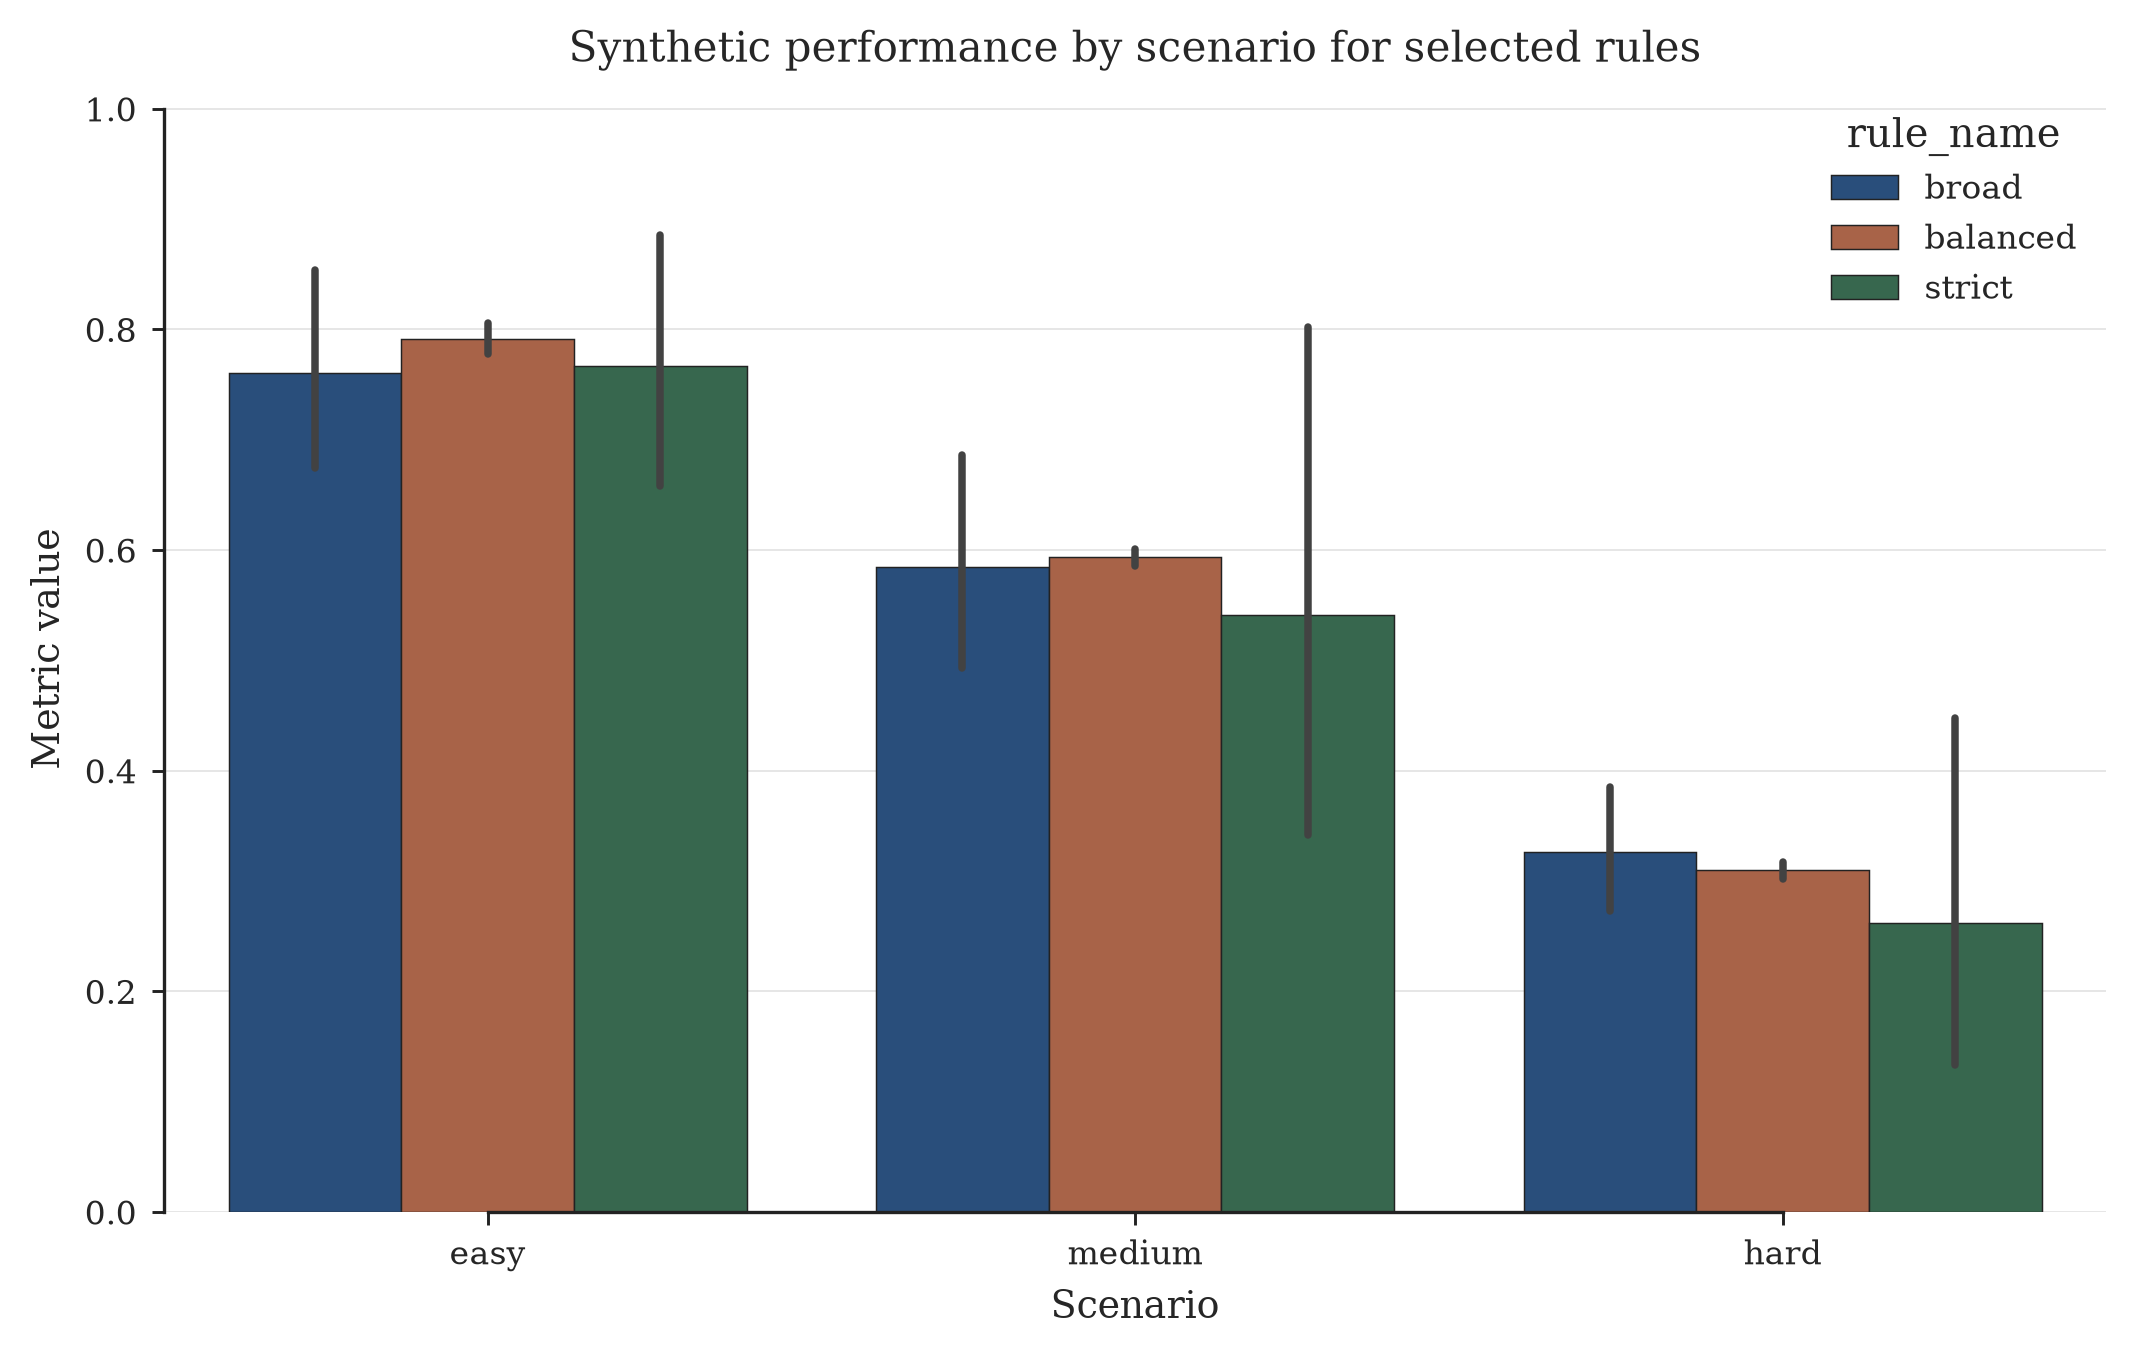
\includegraphics[width=0.92\textwidth]{figures/validation/parameter_selected_rules_scenario_performance}
\caption{Synthetic-benchmark performance of the broad, balanced, and strict
rules across the easy/medium/hard scenarios. All three rules degrade under
harder synthetic noise; the balanced rule was chosen for its stability and its
yield of real events, not because it is the single most precise option on
paper.}
\label{fig:scenario-performance}
\end{figure}

\paragraph{Results after the change.}
Re-applied to real BOAMP, the balanced rule produces \textbf{269 proxy
recurrence events} among 1{,}210 eligible source contracts (\textbf{22.2\%}) ---
down from 665 (55.0\%) under the initial rule. The broad sensitivity gives 490
events (40.5\%); the strict sensitivity gives 79 events (6.5\%, underpowered for
Cox/AFT). Figure~\ref{fig:event-rates} shows this drop in scale.

\begin{figure}[H]
\centering
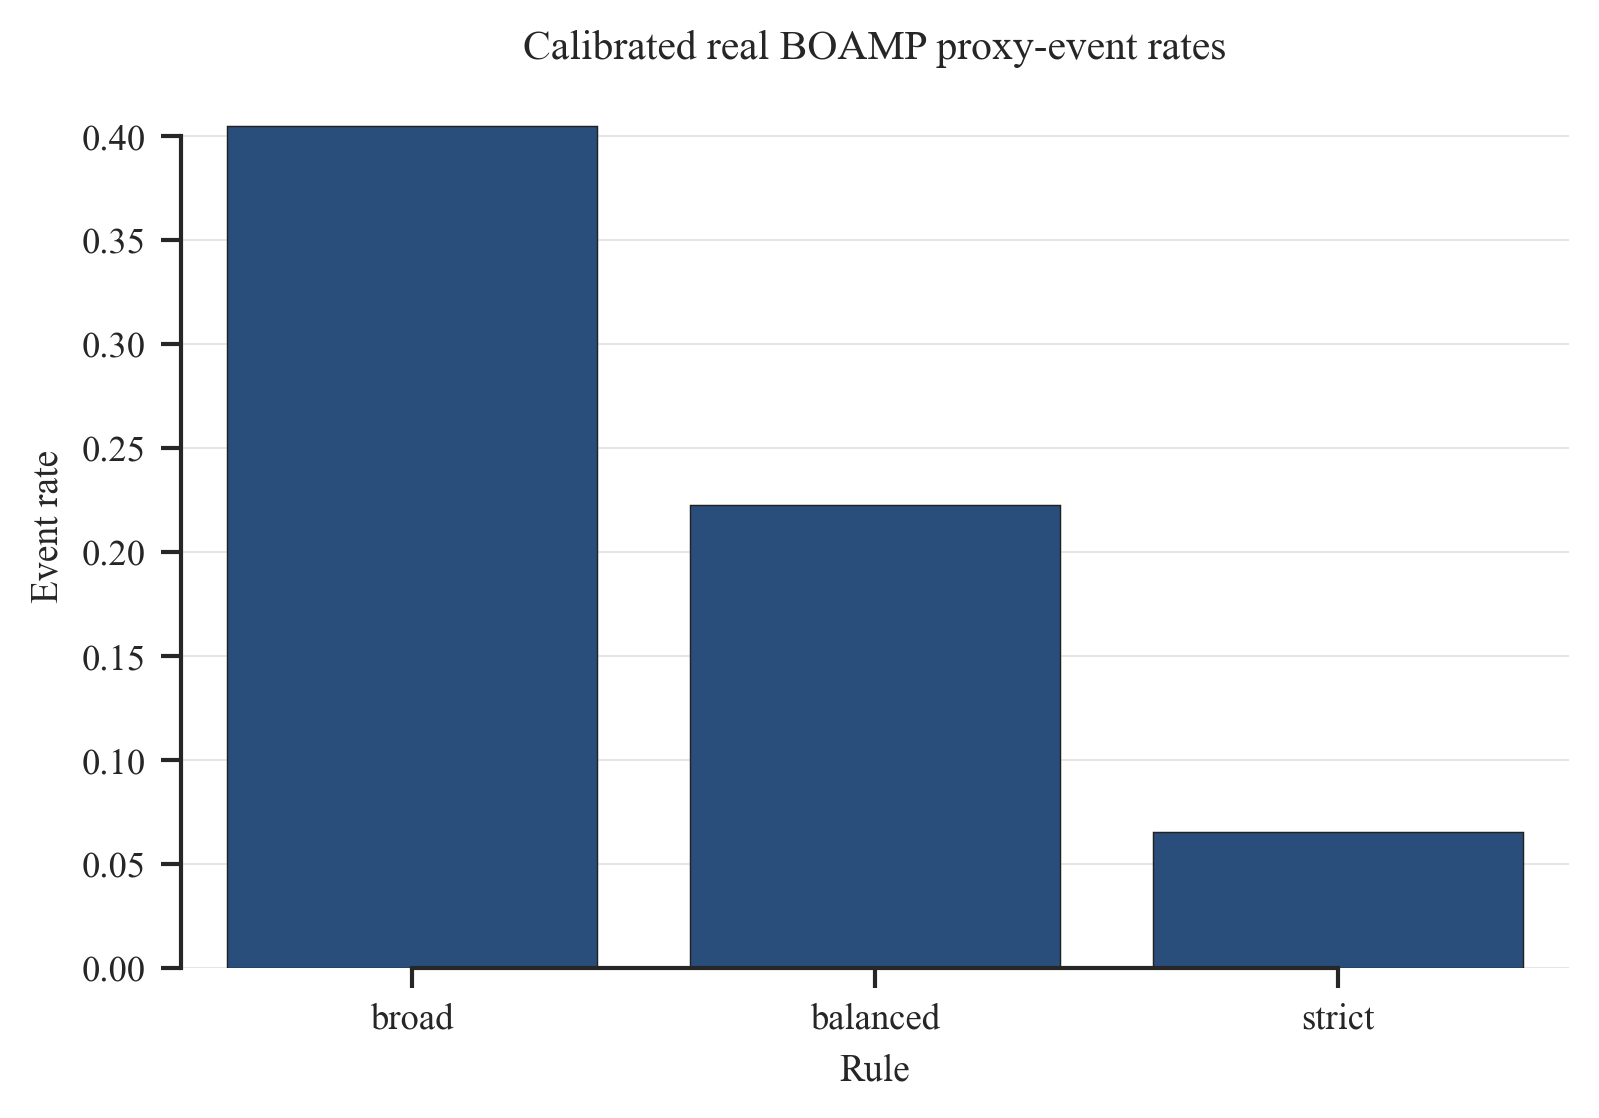
\includegraphics[width=0.7\textwidth]{figures/validation/calibrated_real_event_rates}
\caption{Proxy-event rate on real BOAMP under the three calibrated rules
(1{,}210 eligible contracts). The balanced rule keeps less than half the events
of the broad rule, trading linkage quantity for a rule whose behaviour is
checked on the synthetic benchmark.}
\label{fig:event-rates}
\end{figure}

The calibrated survival-ready file is
\texttt{data/processed/boamp\_phase2\_survival\_calibrated\_balanced.csv}. Its
Kaplan--Meier median is not reached; survival is 95.9\% at 12 months, 92.3\% at
24 months, 83.2\% at 48 months, and 75.2\% at 60 months
(Figure~\ref{fig:km-calibrated}). The Cox C-index is 0.592, and LogNormalAFT is
the best balanced-rule AFT model by AIC (3{,}544.8). Re-scored 12/24-month risk
indicators under this rule give a mean 12-month recurrence probability of 0.023
and 27.5 expected recurrences within 12 months
(\nolinkurl{reports/tables/survival/renewal_risk_12_24_months_calibrated_balanced.csv}).

\begin{figure}[H]
\centering
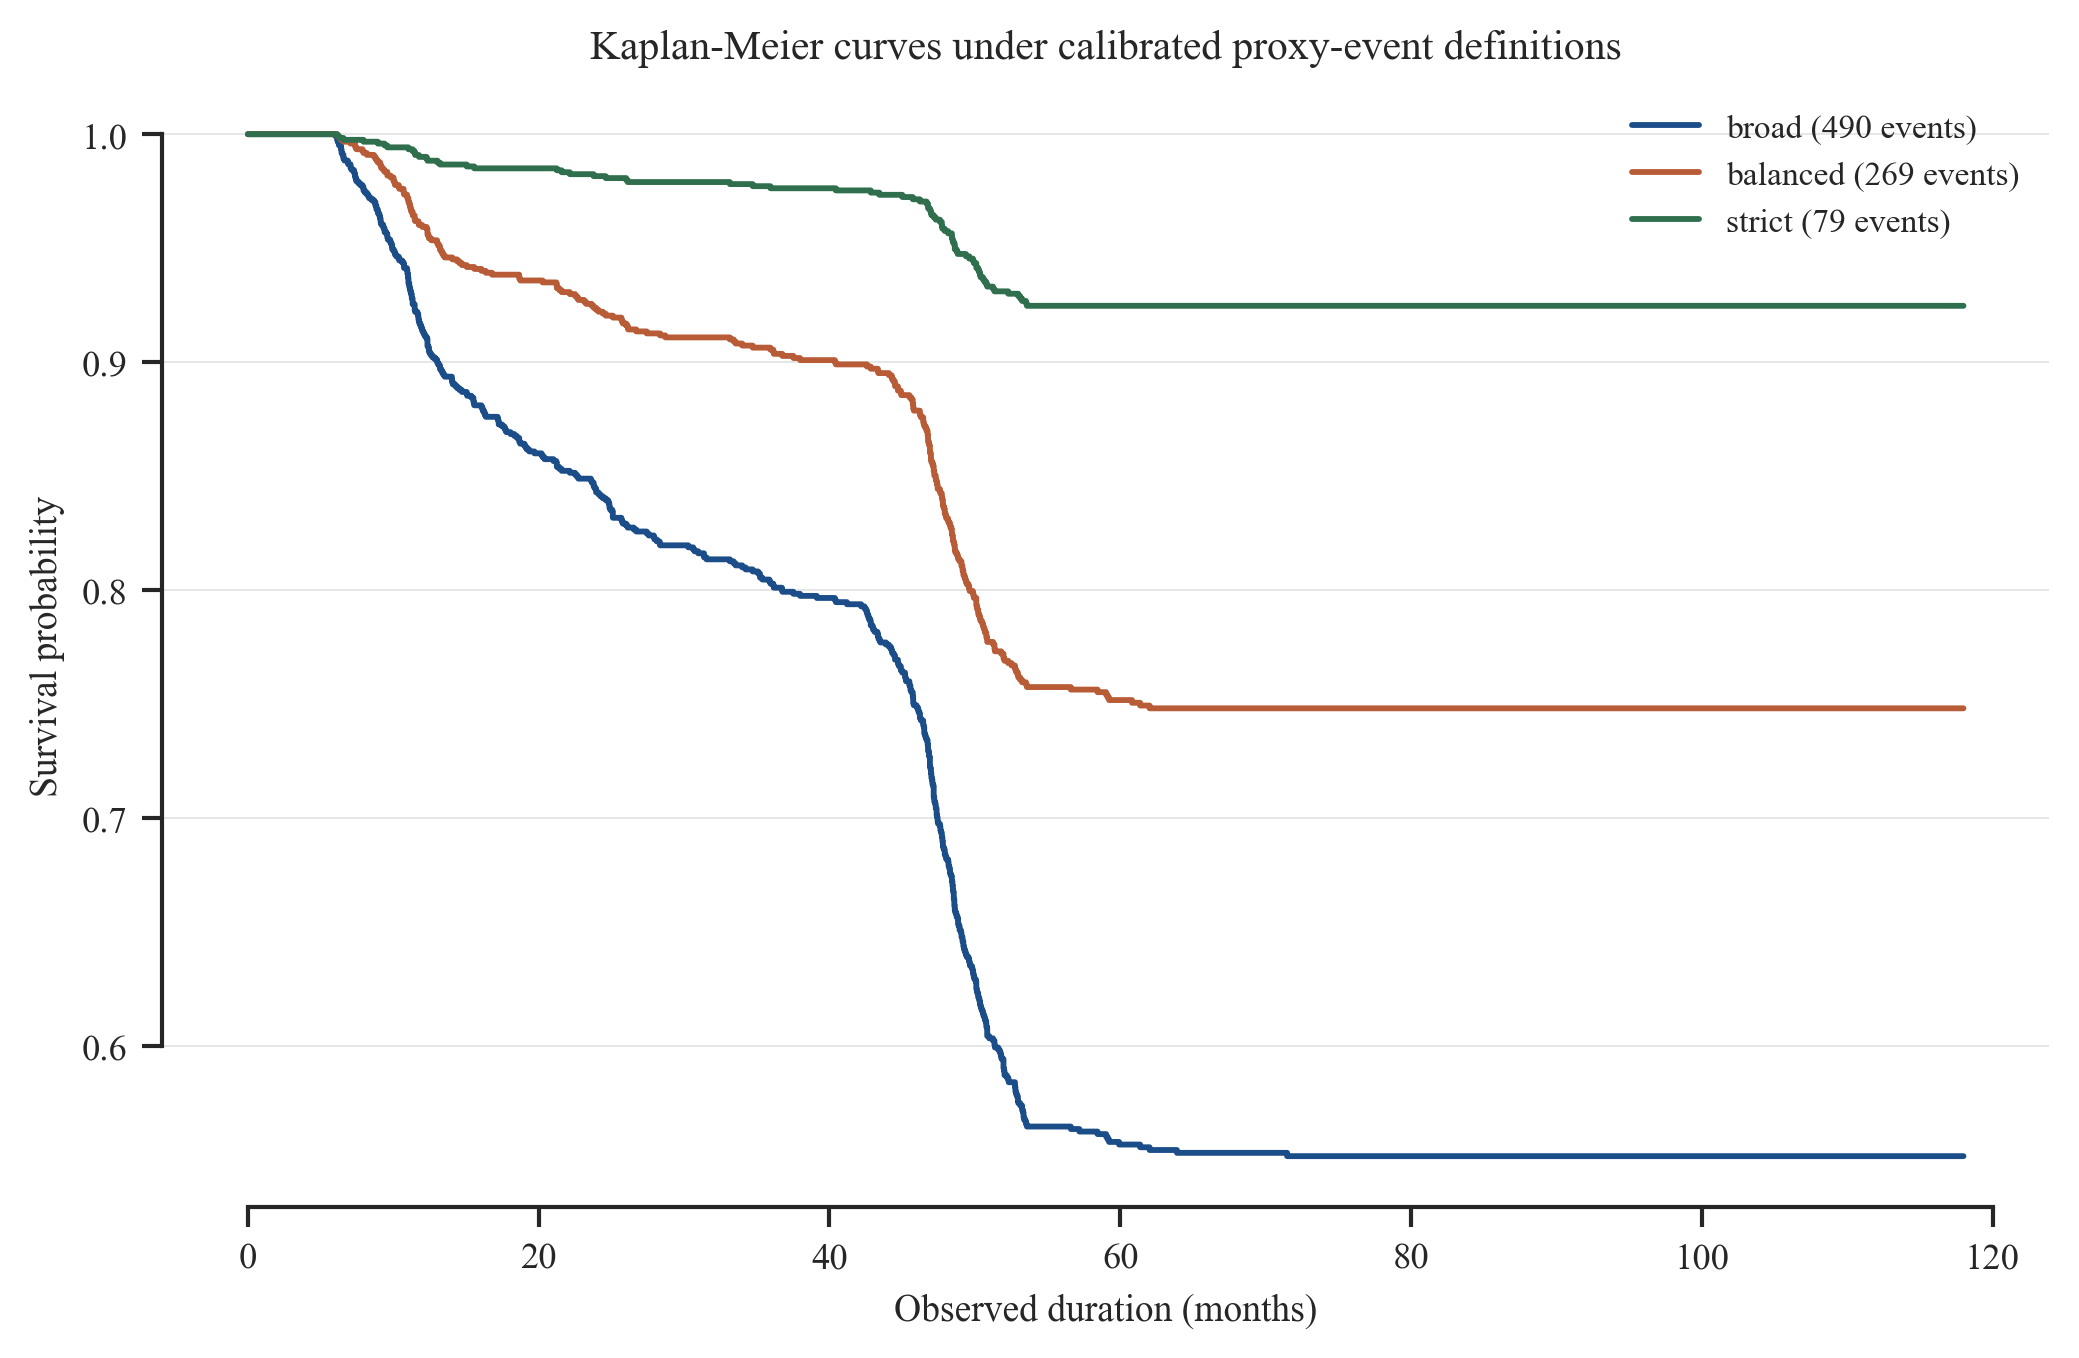
\includegraphics[width=0.85\textwidth]{figures/survival/calibrated_rules_km_curves}
\caption{Kaplan--Meier survival curves under the three calibrated proxy-event
rules. The stricter the rule, the fewer and later the recorded events, and the
higher the residual survival at any horizon --- the balanced curve sits between
the broad and strict extremes, as intended by the calibration.}
\label{fig:km-calibrated}
\end{figure}

\paragraph{Limitation.}
Because BOAMP does not provide an official renewal label, the constructed
\texttt{event} variable --- under any of the three rules --- should be
interpreted as a proxy for \emph{likely procurement recurrence}, not as
verified legal renewal ground truth. The synthetic benchmark quantifies how the
linking method behaves under controlled noise; it does not certify that any
specific real link is a true renewal. These labels remain proxy recurrences,
not legally verified renewals.

\paragraph{Conclusion of this note.}
The methodological change is the main deliverable of the calibration phase: the
project moved from \textbf{maximizing linkage quantity} (665 events, 55.0\%,
uncalibrated) to \textbf{maximizing analytical reliability} (269 events, 22.2\%,
calibrated against a controlled benchmark). The rest of this report documents
both stages so the reader can see what changed and why. The detailed
implementation is reproducible from
\texttt{notebooks/04\_synthetic\_boamp\_benchmark.ipynb} and
\texttt{notebooks/05\_parameter\_calibration\_benchmark\_and\_real.ipynb}, with
generated artifacts tracked under \texttt{data/synthetic/} and
\texttt{reports/tables/validation/}. Section~\ref{sec:reliability} gives the
full manual-audit and robustness evidence behind this decision.

% ===========================================================================
\section{Context and Objective}

\subsection{Why this project}
Gigalis operates a central purchasing body for digital services in Pays de la
Loire. To anticipate re-tendering workloads, it wants to predict \emph{when}
digital contracts come up for renewal. The core obstacle: BOAMP publishes calls
for tenders and awards, but \emph{no notice says ``this renews contract X''}.
The renewal link must be inferred from text, classification, timing, and buyer
identity.

\subsection{Objective}
The internship objective is to build a transparent, reproducible pipeline that
(i) reconstructs a proxy renewal \texttt{event} from BOAMP signals, (ii) uses it
as the outcome of a survival model of contract lifetime, and (iii) translates
the model into operational renewal-risk indicators. This report orients the
reader to that pipeline and its main results; exact field logic, formulas, and
diagnostics are deferred to the technical and data quality reports.

% ===========================================================================
\section{Data Sources and Scope}
\label{sec:data}

\subsection{Scope}
\begin{itemize}[leftmargin=1.4em,itemsep=1pt]
  \item \textbf{Sectors:} CPV divisions 48 (software), 72 (IT services), 32 (telecom), 35 (security).
  \item \textbf{Territory:} departments 44, 49, 53, 72, 85 (Pays de la Loire).
  \item \textbf{Period:} 2015--2024. Study end date: 2024-12-31.
  \item \textbf{Modeling path:} BOAMP only. DECP is documented but not linked
        (no shared key between the two sources).
\end{itemize}

\subsection{Corpus numbers}
\begin{itemize}[leftmargin=1.4em,itemsep=1pt]
  \item 3{,}181 BOAMP notices downloaded (2015--2024).
  \item 1{,}933 are \texttt{APPEL\_OFFRE} (source contracts); 1{,}081 are \texttt{ATTRIBUTION}.
  \item 1{,}210 are \emph{eligible}: their expected renewal window ($\pm 6$ months around the estimated end date) closes before 2024-12-31.
  \item 723 are structurally censored upfront (too recent to observe a renewal).
\end{itemize}

DECP (3{,}039 digital contracts, same scope) is far richer (100\% SIRET, 99.4\%
durations) but cannot be merged to BOAMP at contract level; contract-level DECP
merging remains a future path.

\subsection{Key data quality issues (modeling consequences)}

\begin{table}[H]
\centering
\caption{Key BOAMP data-quality findings and their modeling consequence.
Full field-level detail is in the data quality report.}
\label{tab:dq}
\small
\begin{tabular}{@{}p{4.8cm}p{2.8cm}p{6.0cm}@{}}
\toprule
\textbf{Finding} & \textbf{Value} & \textbf{Consequence} \\
\midrule
Buyer SIRET coverage (raw) & $\sim$9\% of corpus & Grouping uses normalised names; SIREN enrichment later consolidates many (see \S3.2). \\
Amount fill rate (\texttt{APPEL\_OFFRE}) & $\sim$21\% & Amount excluded from linking signals. \\
Declared duration granularity & 69\% at 12/24/36/48 mo & Duration used as a covariate, not as survival target. \\
Imputed durations & 25\% of eligible cohort & Flagged with \texttt{dur\_was\_imputed}; imputation is 48 months. \\
No explicit renewal label & structural & \texttt{event} is a proxy reconstructed by the linking algorithm. \\
\bottomrule
\end{tabular}
\end{table}

\subsection{Taxonomy}
Each contract is tagged with one of eleven technology categories (Software \&
Applications, IT Services \& Consulting, Telecom \& Networks, Cybersecurity,
Cloud \& Infrastructure, Data \& AI, etc.) via a \textbf{deterministic
rule-based mapping} from CPV codes and description keywords. This is \emph{not}
a trained classifier --- the planned NLP classifier was not implemented.
Output: \nolinkurl{data/processed/taxonomy.csv}.

% ===========================================================================
\section{Main Pipeline}
\label{sec:pipeline}

The pipeline runs end to end from raw BOAMP notices to operational risk
indicators. Table~\ref{tab:pipeline} summarises each component and where its
outputs live; the subsections below describe what each stage does, and
Section~\ref{sec:results} reports the numbers.

\begin{landscape}
\begin{table}[p]
\centering
\caption{Component status and key outputs. Status: \textcolor{done}{Done},
\textcolor{partial}{Partial}, \textcolor{notdone}{Not started}.}
\label{tab:pipeline}
\scriptsize
\begin{tabular}{@{}p{4.2cm}p{1.6cm}p{5.4cm}p{10.0cm}@{}}
\toprule
\textbf{Component} & \textbf{Status} & \textbf{Key result} & \textbf{Where} \\
\midrule
Data cleaning \& EDA
  & \textcolor{done}{Done}
  & 3,181 notices $\to$ 1,933 source contracts
  & \nolinkurl{data/processed/boamp_full_clean.csv} \\[3pt]
Buyer SIREN enrichment
  & \textcolor{done}{Done}
  & 724/1,210 eligible rows on a SIREN key
  & \nolinkurl{buyer_siren_enrichment/} \\[3pt]
Renewal linking (event reconstruction)
  & \textcolor{done}{Done}
  & 665/1,210 eligible linked (55.0\%)
  & \nolinkurl{boamp_renewal_linking_quality/} \\[3pt]
Survival dataset construction
  & \textcolor{done}{Done}
  & 1,210 rows $\times$ 33 cols
  & \nolinkurl{data/processed/boamp_phase2_survival.csv} \\[3pt]
Kaplan--Meier \& log-rank
  & \textcolor{done}{Done}
  & Median 50.1 mo; duration significant
  & \nolinkurl{notebooks/02_survival_modeling_boamp.ipynb} \\[3pt]
Cox PH model
  & \textcolor{done}{Done}
  & C-index 0.6317
  & same notebook + \nolinkurl{reports/tables/survival/} \\[3pt]
Parametric AFT models
  & \textcolor{done}{Done}
  & Log-normal best (AIC 7,068.4)
  & same notebook \\[3pt]
Sensitivity analysis
  & \textcolor{done}{Done}
  & Directions stable (A/B); strict variant underpowered
  & \nolinkurl{reports/tables/survival/sensitivity_comparison.csv} \\[3pt]
Robustness checks
  & \textcolor{done}{Done}
  & Placebo, bias check, threshold sweep
  & \nolinkurl{validation_robustness/} \\[3pt]
Operational risk indicators
  & \textcolor{done}{Done}
  & 12/24-mo risk at contract/buyer/segment
  & \nolinkurl{reports/tables/survival/top20_renewal_risk.csv} \\[3pt]
Manual event validation
  & \textcolor{done}{Done}
  & 150 cases audited; precision $\approx$0.09--0.15 (HIGH tier 0.50)
  & \nolinkurl{event_validation/manual_validation_summary.md} \\[3pt]
Trained NLP classifier
  & \textcolor{partial}{Partial}
  & Scaffolding only: annotation sample (350 rows) + training scripts exist; gold labels and training not yet done
  & \nolinkurl{scripts/nlp_*.py}, \nolinkurl{notebooks/03_nlp_classification.ipynb} \\[3pt]
Change-point detection (Phase 4)
  & \textcolor{notdone}{Not done}
  & Scoped but not implemented
  & --- \\
\bottomrule
\end{tabular}
\end{table}
\end{landscape}

\subsection{BOAMP cleaning}
Raw notices are parsed from the BOAMP API, deduplicated, and standardised:
buyer key construction, contract start-date refinement (using
\texttt{ATTRIBUTION} back-references where available), duration cleaning and
imputation (missing eligible durations set to 48 months, flagged), CPV
normalisation, and text normalisation. Output:
\nolinkurl{data/processed/boamp_full_clean.csv}.

\subsection{Buyer SIREN enrichment}
\label{sec:siren}
Because raw SIRET coverage is weak ($\sim$9\% of the corpus), buyers were
initially grouped by normalised name, which fragments a single public entity
across spelling variants. A \textbf{SIREN enrichment step} (completed
\textbf{2026-06-24}) queries the official \emph{API Recherche d'Entreprises} for
each buyer name and, for \textbf{HIGH-confidence matches only}, upgrades the
buyer key from \texttt{NAME:} to \texttt{SIREN:\{9-digit\}}, merging name aliases
of the same legal entity. Of the 1{,}210 eligible contracts, \textbf{724 carry a
SIREN key (plus 2 SIRET) and 484 remain name-keyed}; 275 of 525 unique buyers (52.4\%) matched
with HIGH confidence. Medium/low matches are kept for review but never applied
automatically. Enrichment is a buyer-resolution improvement, \emph{not} ground
truth: rare false merges at HIGH confidence remain possible. Outputs:
\nolinkurl{buyer_siren_enrichment/} and
\nolinkurl{data/processed/boamp_phase2_survival_siren_enriched.csv}.

\subsection{Renewal-event reconstruction}
\label{sec:linking}
Each eligible source contract is matched against later BOAMP notices from the
same buyer using a four-signal composite score: semantic text embeddings
(Sentence-Transformer, \nolinkurl{paraphrase-multilingual-MiniLM-L12-v2}), CPV
hierarchy match, temporal proximity, and buyer-identity agreement (weights
0.40 / 0.25 / 0.20 / 0.15). The best candidate passing the hard text-similarity
filter is selected as the renewal successor and sets \texttt{event}~$=1$;
contracts with no qualifying successor before study end are right-censored
(\texttt{event}~$=0$). See technical report \S5 for the full formula.

\subsection{Survival modeling}
\label{sec:survival}
The survival dataset (\nolinkurl{data/processed/boamp_phase2_survival.csv}) has
one row per eligible contract with observed/censored duration and covariates
(\nolinkurl{declared_duration_months}, \nolinkurl{dur_was_imputed},
\texttt{start\_year}, category, procedure type). Three model families were
fitted in \nolinkurl{notebooks/02_survival_modeling_boamp.ipynb}: Kaplan--Meier
(with log-rank tests), a Cox proportional-hazards model, and parametric AFT
models (Weibull, log-logistic, log-normal). The fitted model was stress-tested
with a sensitivity analysis over three event definitions and a battery of
robustness checks.

\subsection{Operational risk indicators}
\label{sec:operational}
The best parametric model (log-normal AFT) is applied to all scored contracts to
produce conditional renewal probabilities at 12 and 24 months ahead, aggregated
to contract, buyer, and segment level. These are prioritisation indicators, not
legally verified renewal probabilities. Output:
\nolinkurl{reports/tables/survival/top20_renewal_risk.csv}.

% ===========================================================================
\section{Main Results}
\label{sec:results}

\emph{Reading note:} the numbers in this section describe the \textbf{initial}
linking method (broad, uncalibrated, 665 events). They are kept in full because
they show how the method behaves and why it needed calibration. For any
downstream decision, use the \textbf{calibrated balanced rule} (269 events,
22.2\%) from the Methodological Note on p.~1 and Section~\ref{sec:reliability}
instead.

\subsection{Renewal linking}

\begin{table}[H]
\centering
\caption{Renewal-linking outcome.}
\label{tab:link}
\small
\begin{tabular}{@{}lr@{}}
\toprule
\textbf{Quantity} & \textbf{Value} \\
\midrule
Source contracts (\texttt{APPEL\_OFFRE}) & 1{,}933 \\
Eligible (renewal window observable) & 1{,}210 \\
Linked renewals (\texttt{event}~$=1$) & 665 \quad(55.0\%) \\
Right-censored (\texttt{event}~$=0$) & 545 \quad(45.0\%) \\
Lexical baseline linking rate ($W=6$) & 7.6\% \\
\bottomrule
\end{tabular}
\end{table}

Linking rate by category (Table~\ref{tab:bycat}): Software \& Applications and
IT Services \& Consulting renew most (62.8\%, 60.5\%); Data \& AI and IT Hardware
\& Equipment least (30.0\%, 34.6\%). Small categories ($n < 10$) are underpowered.

\begin{table}[H]
\centering
\caption{Event rate by technology category (1{,}210 eligible contracts; events sum to 665).}
\label{tab:bycat}
\small
\begin{tabular}{@{}lrrr@{}}
\toprule
\textbf{Category} & \textbf{n} & \textbf{events} & \textbf{rate \%} \\
\midrule
IT Services \& Consulting          & 344 & 208 & 60.5 \\
Software \& Applications           & 223 & 140 & 62.8 \\
Telecom \& Networks                & 223 & 116 & 52.0 \\
Cybersecurity                      & 136 &  73 & 53.7 \\
Unknown                            & 115 &  49 & 42.6 \\
Digital Workplace \& Collaboration &  51 &  32 & 62.7 \\
Data \& AI                         &  40 &  12 & 30.0 \\
IT Maintenance \& Support          &  22 &  11 & 50.0 \\
IT Hardware \& Equipment           &  26 &   9 & 34.6 \\
Cloud \& Infrastructure            &  22 &  11 & 50.0 \\
GIS \& Mapping                     &   8 &   4 & 50.0 \\
\bottomrule
\end{tabular}
\end{table}

\textbf{Link quality.} Of the 665 accepted links: 164 are single-candidate
(no competing match); of the remaining 501 multi-candidate links, 219 (44\%)
have a score margin below 0.05, flagging an ambiguous winner. 75 links (11.3\%)
satisfy the \texttt{high\_confidence\_strict} criterion ($S \geq 0.70$ and margin
$\geq 0.05$, multi-candidate only); these form the Model~C core
(Table~\ref{tab:sens}). \textbf{Main unlinked failure mode:} 491 of 545 unlinked
contracts (90.1\%) have no temporal partner in the search window --- a true absence
of a candidate notice, not a scoring failure.

\subsection{Survival analysis}

\paragraph{Kaplan--Meier.} Global median survival is \textbf{50.1 months},
consistent with the prevalence of 48-month framework contracts. Log-rank tests
(Table~\ref{tab:logrank}): renewal timing is driven by declared duration and
imputation status ($p<0.001$); category is marginally significant ($p=0.025$).

\begin{table}[H]
\centering
\caption{Log-rank tests for differences in renewal timing.}
\label{tab:logrank}
\small
\begin{tabular}{@{}lrrr@{}}
\toprule
\textbf{Stratifying variable} & \textbf{statistic} & \textbf{p} & \textbf{df} \\
\midrule
Category (multivariate)        & 12.89 & 0.025 & 5 \\
Duration was imputed           & 19.96 & $<0.001$ & 1 \\
Declared-duration group        & 41.05 & $<0.001$ & 2 \\
Procedure type (collapsed)     &  3.48 & 0.176 & 2 \\
\bottomrule
\end{tabular}
\end{table}

\paragraph{Cox proportional-hazards model.} In-sample concordance:
\textbf{0.6317}. Two predictors are significant (Table~\ref{tab:cox}): longer
declared duration lowers hazard (HR 0.991 per month), and later start year
raises it (HR 1.071 per year). IT Services \& Consulting shows a positive
category effect (HR 1.230, $p=0.037$). The positive
\texttt{start\_year} hazard is partly structural: 2021--2024 contracts are
right-censored because a typical 48-month contract would renew after the
2024-12-31 study close.

\begin{table}[H]
\centering
\caption{Cox model: significant covariates (multivariate).}
\label{tab:cox}
\small
\begin{tabular}{@{}lrrr@{}}
\toprule
\textbf{Covariate} & \textbf{HR} & \textbf{95\% CI} & \textbf{p} \\
\midrule
\texttt{declared\_duration\_months} & 0.991 & [0.986, 0.995] & $<0.001$ \\
\texttt{start\_year}                & 1.071 & [1.031, 1.113] & $<0.001$ \\
IT Services \& Consulting (vs.\ Cybersecurity) & 1.230 & [1.013, 1.493] & 0.037 \\
\texttt{dur\_was\_imputed}          & 0.871 & [0.722, 1.049] & 0.146 \\
Other category / procedure terms    & \multicolumn{3}{c}{not significant ($p>0.1$)} \\
\bottomrule
\end{tabular}
\end{table}

\paragraph{Parametric AFT models.} Log-normal fits best (AIC 7{,}068.4,
concordance 0.655), outperforming log-logistic (7{,}154.7) and Weibull
(7{,}240.3). Full results:
\nolinkurl{reports/tables/survival/parametric_aic_comparison.csv}.

\paragraph{Sensitivity to event definition.} Three event definitions were tested
(Table~\ref{tab:sens}). The Cox concordance drops from 0.632 (Model A) to 0.616
(Model B, $\geq$0.50) and 0.455 (Model C, strict H.C.), suggesting that
low-confidence links add predictive signal not present in the strict subset ---
and that the 75-event strict definition is too sparse for stable estimation.

\begin{table}[H]
\centering
\caption{Sensitivity to event definition. ``--'' = KM median never reached.
KM median in months.}
\label{tab:sens}
\small
\begin{tabular}{@{}lrrrr@{}}
\toprule
\textbf{Variant} & \textbf{events} & \textbf{rate \%} & \textbf{KM median} & \textbf{Cox C} \\
\midrule
A --- baseline (all links)            & 665 & 55.0 & 50.1 & 0.632 \\
B --- conservative ($\geq 0.50$)      & 400 & 33.1 & -- & 0.616 \\
C --- strict H.C.\ ($S\!\geq\!0.70$, $\Delta\!\geq\!0.05$, multi-cand.) &  75 & 6.2 & -- & 0.455 \\
\bottomrule
\end{tabular}
\end{table}

\paragraph{Proportional-hazards assumption.} The Schoenfeld test flags a
violation for \nolinkurl{declared_duration_months} ($p < 10^{-5}$); all other
covariates pass. Stratification or a time interaction for duration is future
work. The log-normal AFT avoids the PH assumption and gives the same conclusions.

\paragraph{Temporal hold-out.} A temporal validation (train on contracts
starting $\leq$2021: 1{,}088 rows / 604 events; test on $\geq$2022: 116 rows /
60 events) gives a test concordance of 0.543 against 0.612 in-sample ---
a directional check only, since the small test cohort is structurally dominated
by early renewals, but it confirms the in-sample C-index is an upper bound.

\subsection{Operational risk indicators}

The table below is computed under the \emph{pre-calibration} baseline event
definition (665 events). Under the calibrated balanced rule (269 events; see
the calibration update on p.~1), the re-scored indicators are substantially
lower: mean 12/24-month probabilities 0.023/0.068, max 12-month probability
0.073, and 27.5 expected recurrences within 12 months (83\% lower than the
89.7 below). Files: \nolinkurl{reports/tables/survival/*_calibrated_balanced.csv}.

\begin{table}[H]
\centering
\caption{Operational risk summary (1{,}204 scored contracts).}
\label{tab:risk}
\small
\begin{tabular}{@{}lr@{}}
\toprule
\textbf{Metric} & \textbf{Value} \\
\midrule
Mean 12-month renewal probability & 0.074 \\
Mean 24-month renewal probability & 0.216 \\
Max 12-month probability (any contract) & 0.288 \\
Contracts in \emph{medium} band (0.25--0.50) & 6 \\
Contracts in \emph{low} band ($<0.25$) & 1{,}198 \\
Expected renewals within 12 months & 89.7 \\
Expected renewals within 24 months & 259.9 \\
Top buyer by expected 12-month volume & SIREN:234400034 (9.3) \\
Top segment by expected 12-month volume & IT Services \& Consulting (30.4) \\
\bottomrule
\end{tabular}
\end{table}

% ===========================================================================
\section{Reliability and Limitations}
\label{sec:reliability}

\subsection{Reliability evidence}
The event variable was stress-tested with checks in \nolinkurl{validation_robustness/}:
\begin{itemize}[leftmargin=1.4em,itemsep=1pt]
  \item \textbf{Threshold sensitivity (7 scenarios: baseline, composite floors
        0.50--0.90, strict H.C.):} Cox concordance declines gradually from 0.632
        (baseline) to 0.599 (score $\geq 0.60$), then becomes unstable below
        $\approx$100 events (0.473 at $\geq 0.70$); hazard-ratio directions stay
        stable at every threshold with enough events.
        Full table: \nolinkurl{validation_robustness/outputs/threshold_sensitivity_summary.csv}.
  \item \textbf{Placebo check:} winning-link mean score 0.554 vs.\ runner-up
        0.428 vs.\ synthetic no-buyer 0.401 --- the scoring discriminates
        (14.9\% of winners reach $\geq 0.70$ vs.\ 0.7\% of runner-ups).
  \item \textbf{Event/censoring bias:} SMD = 0.17 (duration), $-$0.15 (start year)
        between event and censored groups --- covariates reasonably balanced
        (SMD $<$ 0.20); the dominant bias is structural right-censoring of
        2022--2024 contracts.
  \item \textbf{Manual validation (executed 2026-07-02):} 150 stratified cases
        audited against the full official BOAMP records
        (\nolinkurl{event_validation/outputs/manual_validation_audit_labeled.csv}).
        Result: TP 14 / FP 82 / uncertain 4 on 100 linked pairs
        (precision $\approx$0.15 raw, $\approx$0.09 weighted to the 665-event
        population; 0.50 in the HIGH/strict tier; 1.00 at text similarity
        $\geq$0.80); 6 of 47 decided unlinked sources hid a plausible missed
        renewal (12.8\%). This is a sample-based audit estimate, not
        population ground truth; it invalidates the LOW tier and weakens the
        MEDIUM tier as renewal evidence.
\end{itemize}

\subsection{Key limitations}
\begin{itemize}[leftmargin=1.4em,itemsep=2pt]
  \item \textbf{Proxy event, not legal ground truth.} Because BOAMP does not
        provide an official renewal label, the constructed \texttt{event}
        variable should be interpreted as a proxy for likely procurement
        recurrence, not as verified legal renewal ground truth --- under the
        initial rule (\texttt{event = 1} means a plausible renewal link was
        found; by composite score, 39.8\% of the 665 links are below 0.50 (low),
        45.3\% between 0.50 and 0.70 (medium), 14.9\% at or above 0.70 (high))
        and equally under the calibrated balanced rule.
  \item \textbf{Residual buyer fragmentation.} SIREN enrichment consolidated 724
        of the 1{,}210 eligible rows onto a SIREN key (plus 2 SIRET), but 484 remain
        name-keyed, so spelling variants not resolved by the API can still create
        false negatives. Enrichment is not ground truth.
  \item \textbf{Short-text false positives.} Generic descriptions
        (``prestations informatiques'') can match spuriously.
  \item \textbf{Structural right-censoring.} Contracts from 2021--2024 are largely
        censored; the positive start\_year hazard partly reflects study truncation,
        not a genuine cohort trend.
  \item \textbf{Modest discrimination.} Concordance $\approx$0.65 --- useful for
        prioritisation, not sufficient for high-stakes individual decisions.
\end{itemize}

% ===========================================================================
\section{Completed Work and Remaining Work}
\label{sec:open}

\textbf{Completed.} BOAMP acquisition and cleaning; buyer SIREN enrichment
(2026-06-24); pre-calibration renewal-event reconstruction (665 events,
55.0\%); synthetic benchmark calibration with the real Sentence-Transformer
encoder; calibrated balanced event definition (269 events, 22.2\%); calibrated
survival rerun (KM, Cox, AFT); operational 12/24-month risk indicators
(pre-calibration and re-scored calibrated versions); rule-based technology
taxonomy.

\textbf{Remaining.}
\begin{itemize}[leftmargin=1.4em,itemsep=2pt]
  \item \textbf{Use the calibrated event definition.} The 150-case audit
        (executed 2026-07-02) showed that the broad baseline was too permissive.
        The priority is now to use the balanced calibrated dataset as the main
        survival input and keep broad/strict variants as sensitivity checks.
  \item \textbf{Trained NLP classifier.} The technology taxonomy is rule-based
        (CPV + keywords). The classifier pipeline is scaffolded
        (\nolinkurl{scripts/nlp_annotation_sample.py} through
        \nolinkurl{scripts/nlp_propagate_labels.py} and notebook 03), and the
        350-row annotation sample is drawn, but the gold labels have not been
        filled in and no model has been trained yet.
  \item \textbf{Change-point / trend detection (Phase 4).} Scoped but not started.
  \item \textbf{DECP semantic linking.} Applied to BOAMP only; DECP linking remains
        at the lexical prototype stage.
  \item \textbf{Live prediction scoring.} The current model evaluates contract age
        as of the study end date; a production run would re-evaluate each contract
        at a live prediction date.
\end{itemize}

% ===========================================================================
\section{Conclusion and Next Steps}

The internship delivered a reproducible end-to-end pipeline: BOAMP notice
acquisition $\to$ cleaning $\to$ buyer SIREN enrichment $\to$ renewal-event
reconstruction $\to$ survival modeling $\to$ operational risk indicators. The
main methodological result is not a single number but a \textbf{change in
method}: the project moved from an initial rule that maximized \emph{linkage
quantity} (665 events, 55.0\%, later shown by manual audit to be only
$\approx$9--15\% precise) to a calibrated proxy-event definition that maximizes
\textbf{analytical reliability} against a controlled synthetic benchmark ---
the broad rule gives 490 events (40.5\%), the balanced rule gives 269 events
(22.2\%), and the strict rule gives 79 events (6.5\%). Under the balanced rule,
the Kaplan--Meier median is not reached and LogNormalAFT is the best AFT model
by AIC (3{,}544.8). These outputs translate BOAMP proxy recurrence signals ---
not verified legal renewals --- into 12/24-month renewal-risk rankings.

\textbf{Immediate next steps (prioritised):}
\begin{enumerate}[leftmargin=1.4em,itemsep=2pt]
  \item \textbf{Run the next survival interpretation on the balanced dataset.}
        Use broad and strict only as sensitivity checks; do not report real
        precision/recall without manual labels.
  \item \textbf{Re-score contracts at a live prediction date} (current scores use
        end-of-study ages).
  \item \textbf{Review medium/low SIREN matches} to extend buyer consolidation
        beyond the 724 HIGH-confidence rows already applied.
  \item \textbf{Replace the rule-based taxonomy} with a trained text classifier.
  \item \textbf{Implement change-point detection} (Phase 4).
\end{enumerate}

\end{document}
